\documentclass[a4paper,titlepage,10pt]{article}
\usepackage[margin=0.5in]{geometry}
\usepackage[spanish]{babel} % Le indicamos a LaTeX que vamos a escribir en espa�ol.
\usepackage[latin1]{inputenc} % Permite utilizar tildes y e�es normalmente
%\usepackage{framed}
\usepackage{caratula}
\usepackage{verbatim}

\titulo{Trabajo Pr�ctico 1\\Carpooling}
\fecha{19 / 09 / 2012}
\materia{Ingenier�a De Software 1}
\grupo{Grupo 1}
\integrante{Browarnik, Mart�n}{04/10}{mibrowar0@gmail.com}
\integrante{Carreiro, Mart�n}{45/10}{martin301290@gmail.com}
\integrante{Kujawski, Kevin}{459/10}{kevinkuja@gmail.com}
\integrante{Ortiz de Zarate, Juan Manuel}{403/10}{jmanuoz@gmail.com}
\integrante{Soifer, Alexis}{25/10}{alex1879@gmail.com}
\begin{document} 

\maketitle

\section{Aclaraciones} %Decisiones tomadas por el grupo
Queremos aclarar que las flechas de las nubes O-refinamiento deber�an salir de las flechas de los objetivos pero el programa que utilizamos no permit�a esta opci�n.

\subsection{Selecci�n y Acpetaci�n} %Agregra una subseccion por tema
\begin{itemize}
\item El sistema sabe si el pasajero y conductor tuvieron acuerdo ya que en la base de datos se guarda la seleccion del pasajero y luego la aceptaci�n del conductor.
\item Cuando un conductor califica al pasajero esta informaci�n se guarda en la base de datos
\item El conductor acepta al pasajero a traves de una pantalla en la que visualiza todas las solicitudas para los viajes ingresados por �l.
\end{itemize}


\section{Diagrama de Contexto} %Poner imagenes de contexto

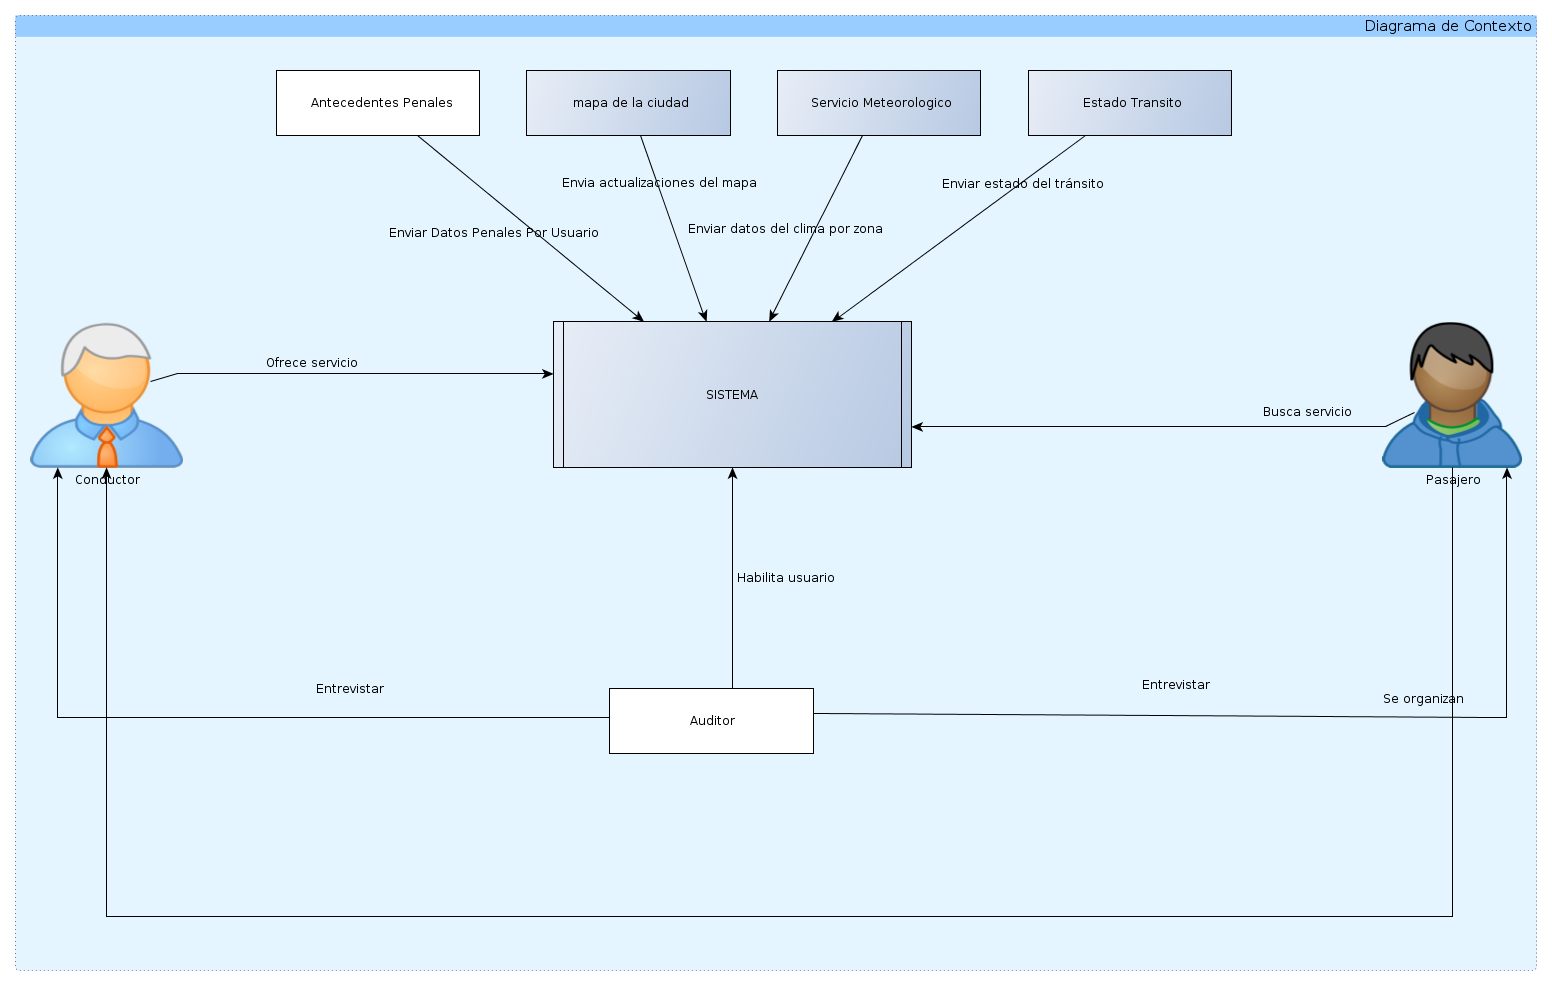
\includegraphics[height=7cm,width=17cm]{imagenes/contexto.png}

\newpage

\section{Diagrama de Objetivos} %Poner imagenes de objetivos
a\\
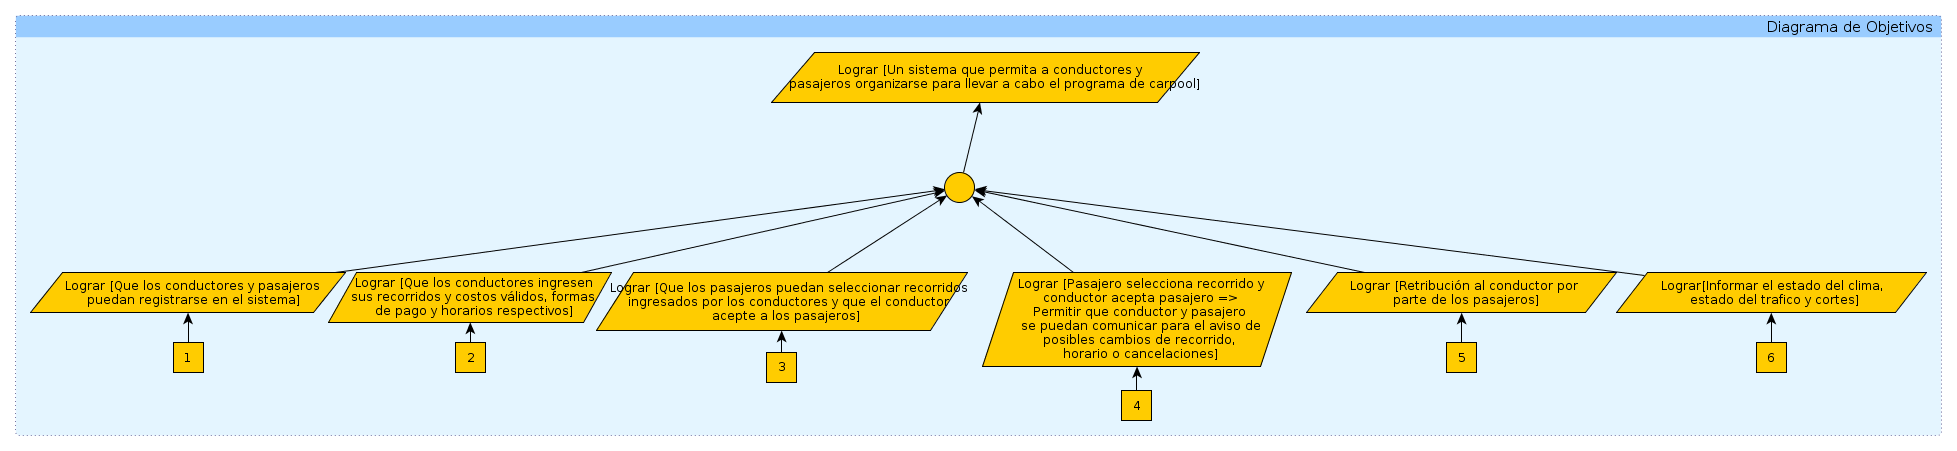
\includegraphics[height=7cm,width=19.5cm]{imagenes/root.png}

\subsection{Registrarse}
a\\
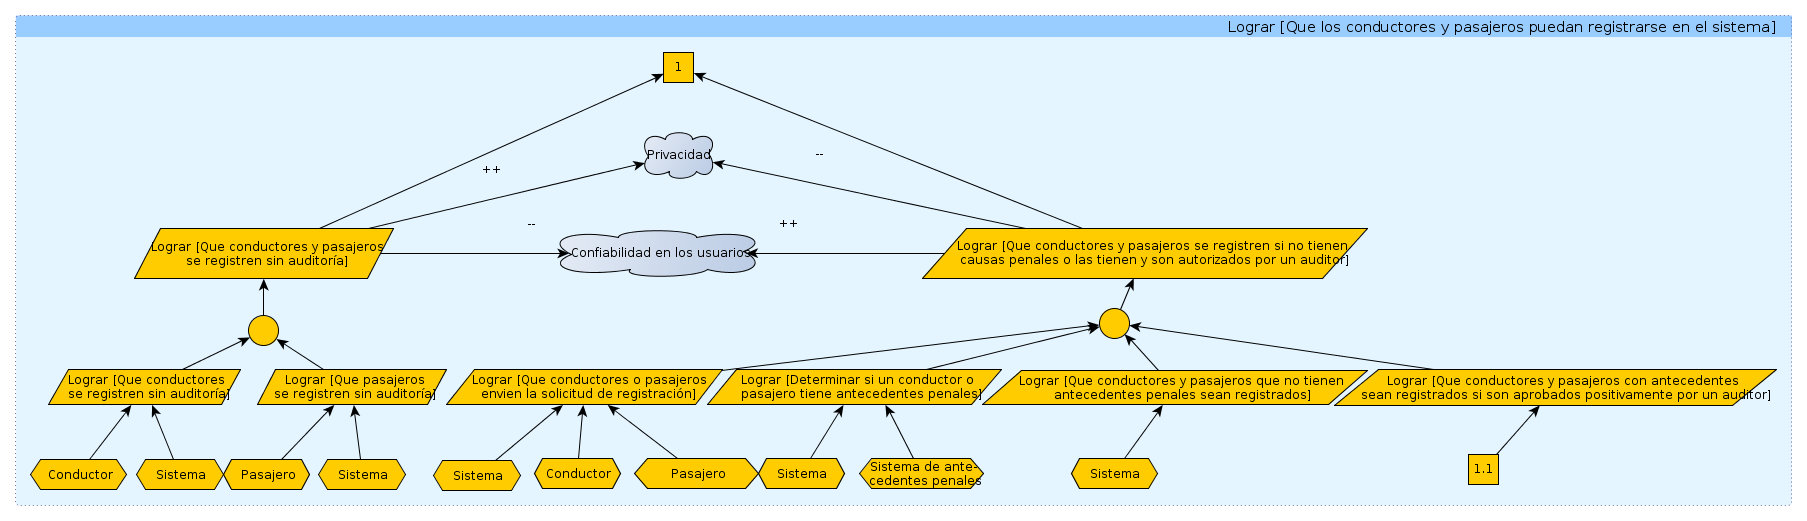
\includegraphics[height=7cm,width=19.5cm]{imagenes/Registrarse.png}
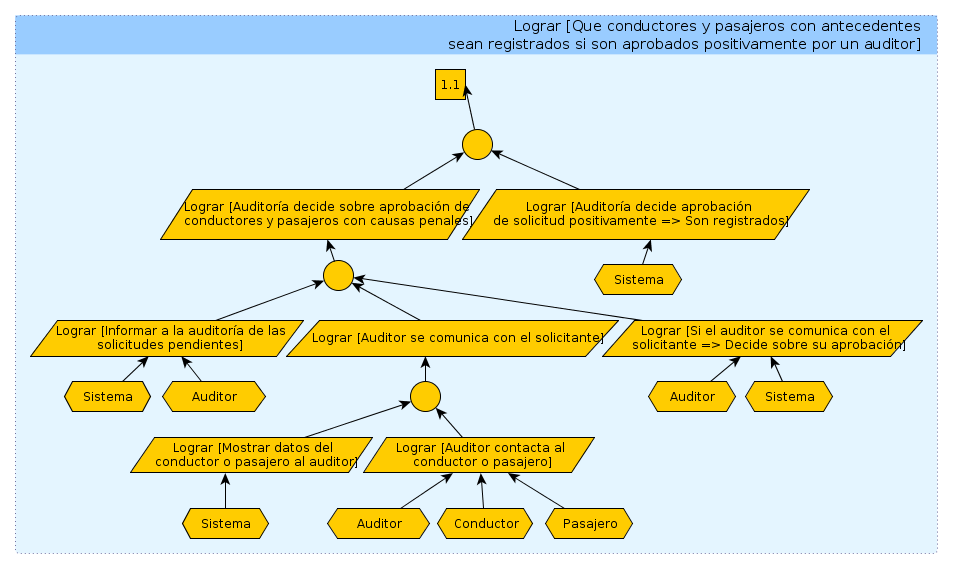
\includegraphics[height=7cm,width=19.5cm]{imagenes/Registrarsea.png}

\subsection{Ingresar Datos}
a\\
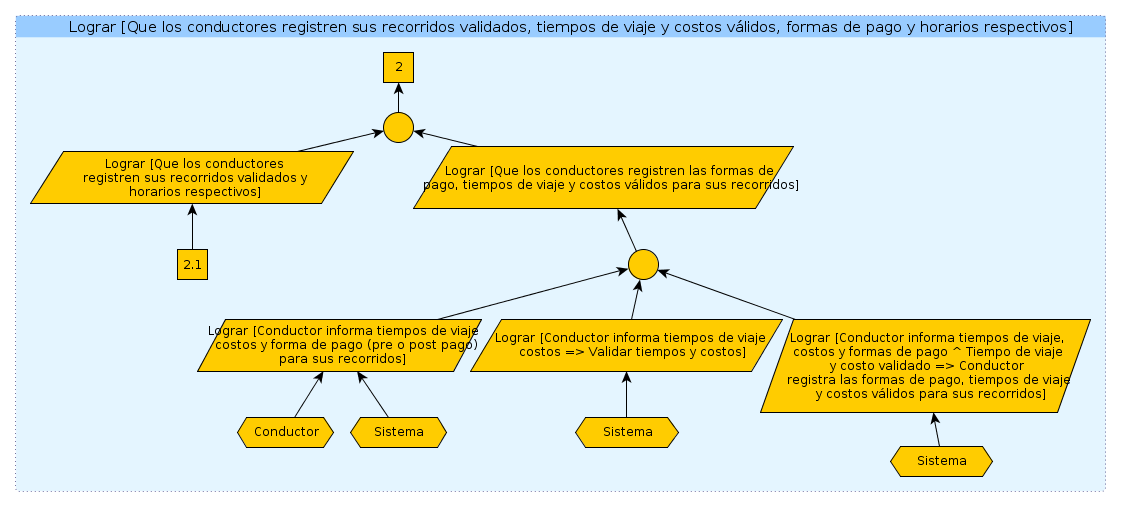
\includegraphics[height=7cm,width=19.5cm]{imagenes/Ingresenrecorridos.png}
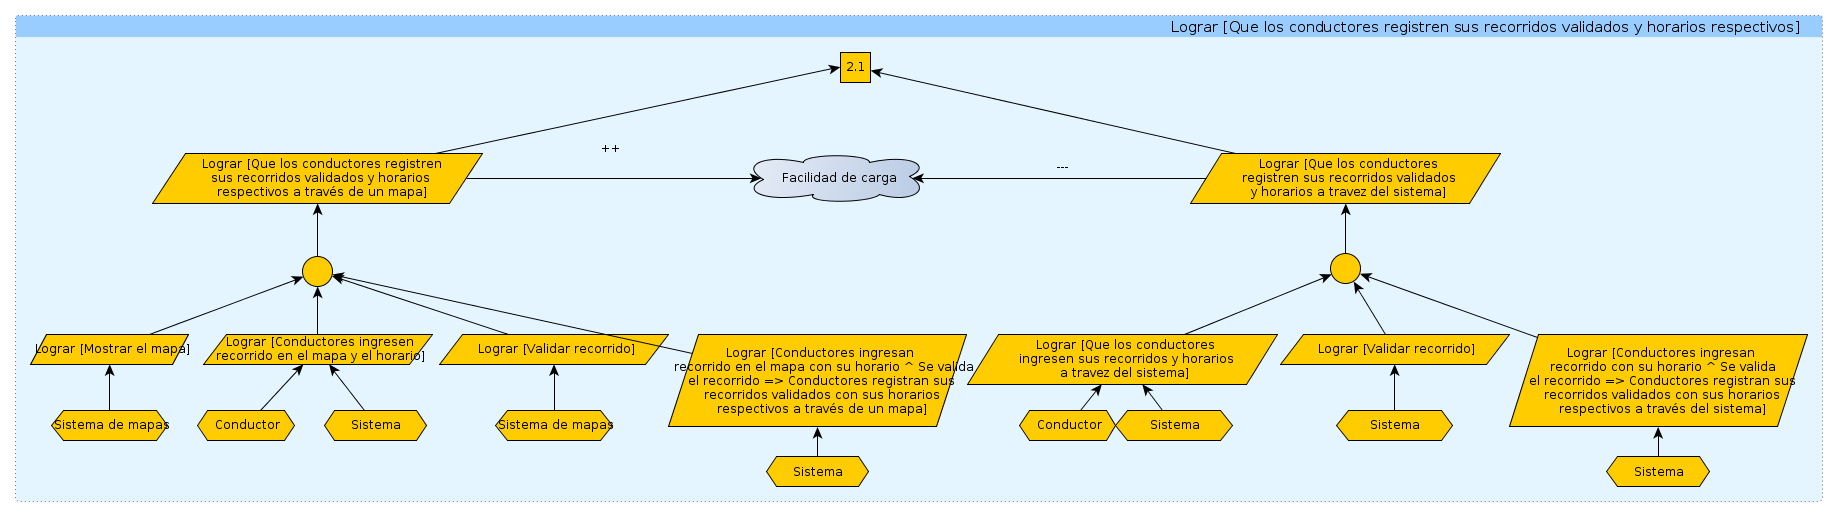
\includegraphics[height=7cm,width=19.5cm]{imagenes/Ingresenrecorridosa.png}

\subsection{Seleccionar Recorrido y Aceptar}
a\\
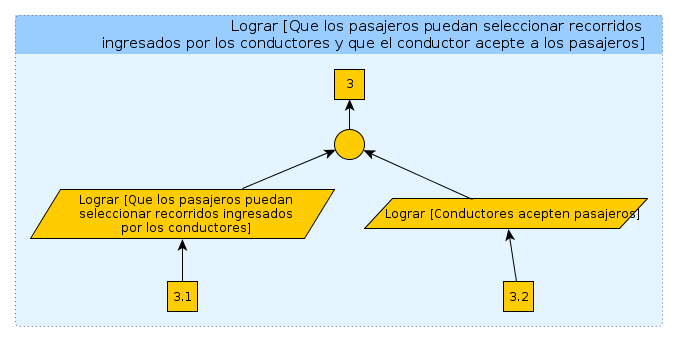
\includegraphics[height=7cm,width=19.5cm]{imagenes/Mostrar.png}
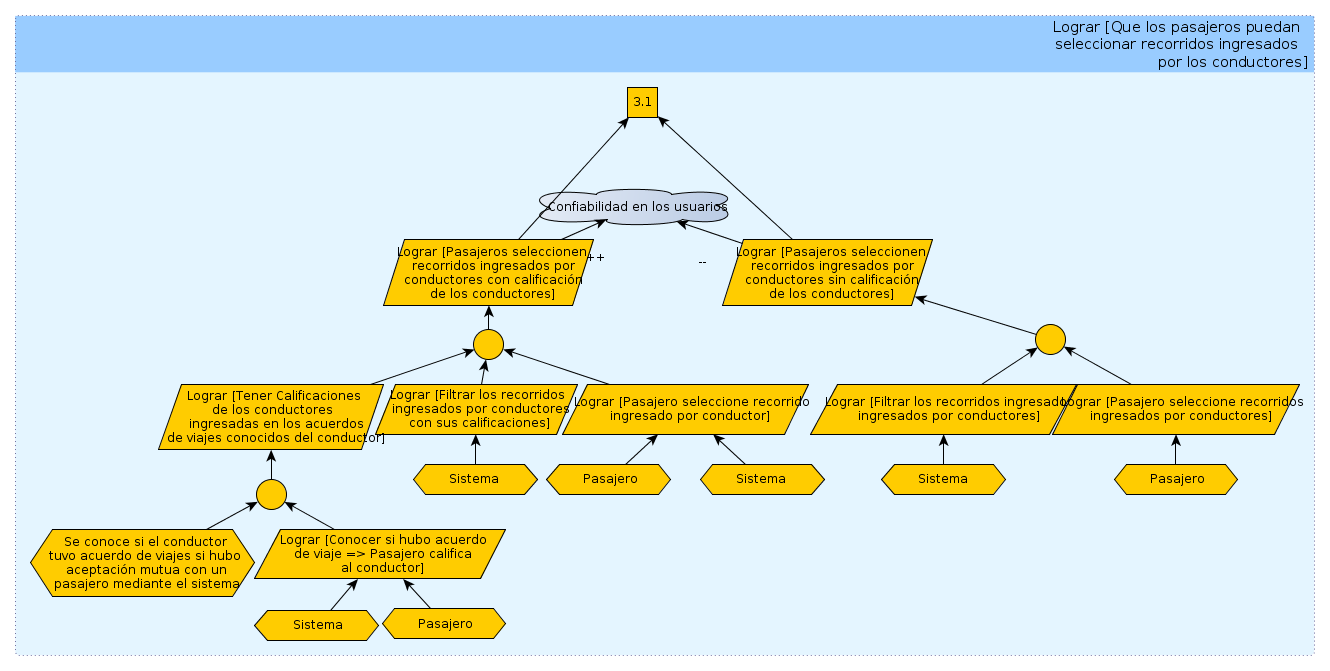
\includegraphics[height=7cm,width=19.5cm]{imagenes/Mostrara.png}
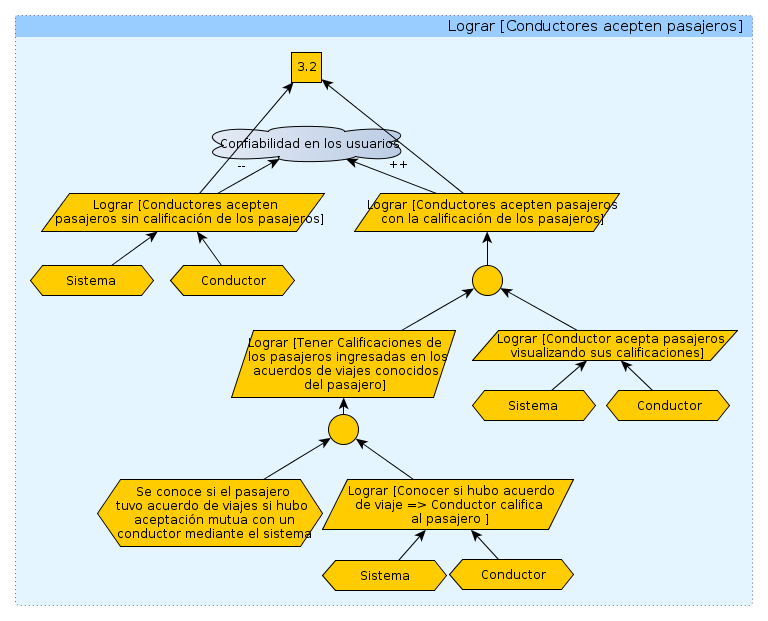
\includegraphics[height=7cm,width=19.5cm]{imagenes/Mostrarb.png}

\subsection{Comunicaci�n}
a\\
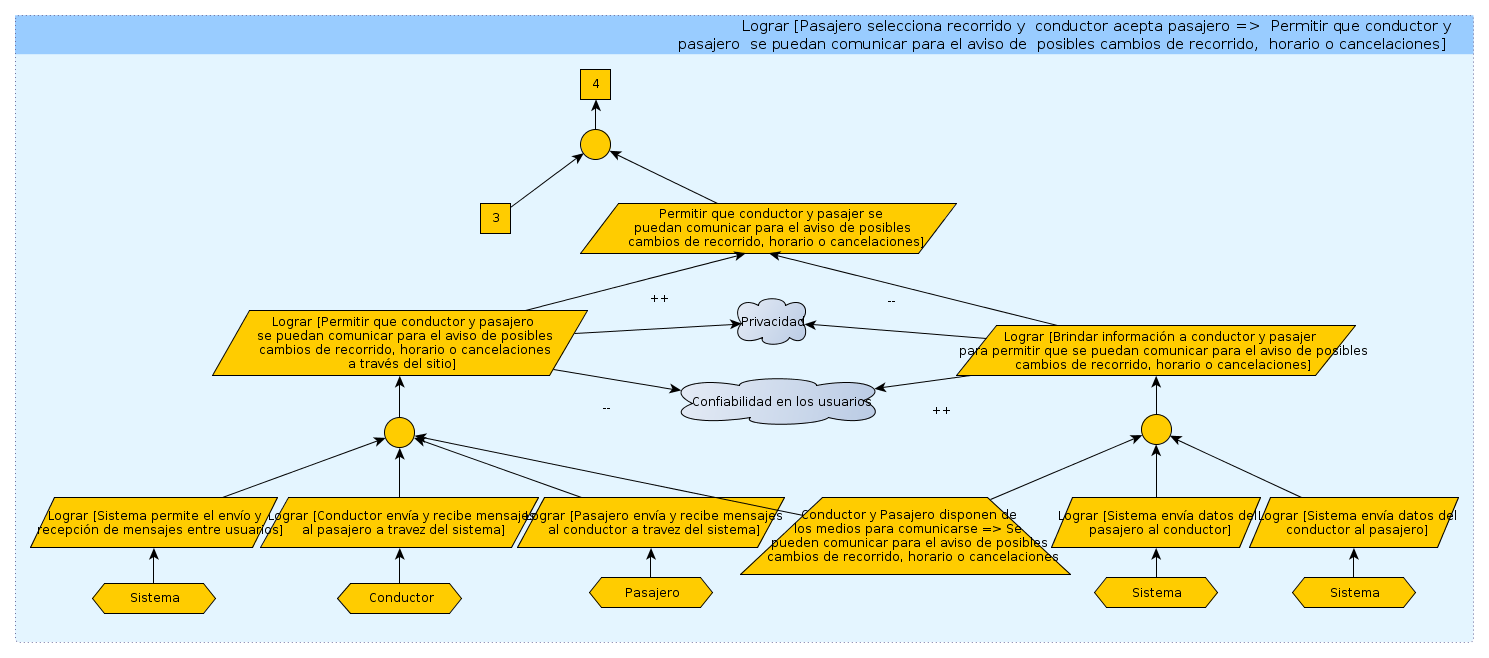
\includegraphics[height=7cm,width=19.5cm]{imagenes/Comunicacion.png}

\subsection{Retribuci�n}
a\\
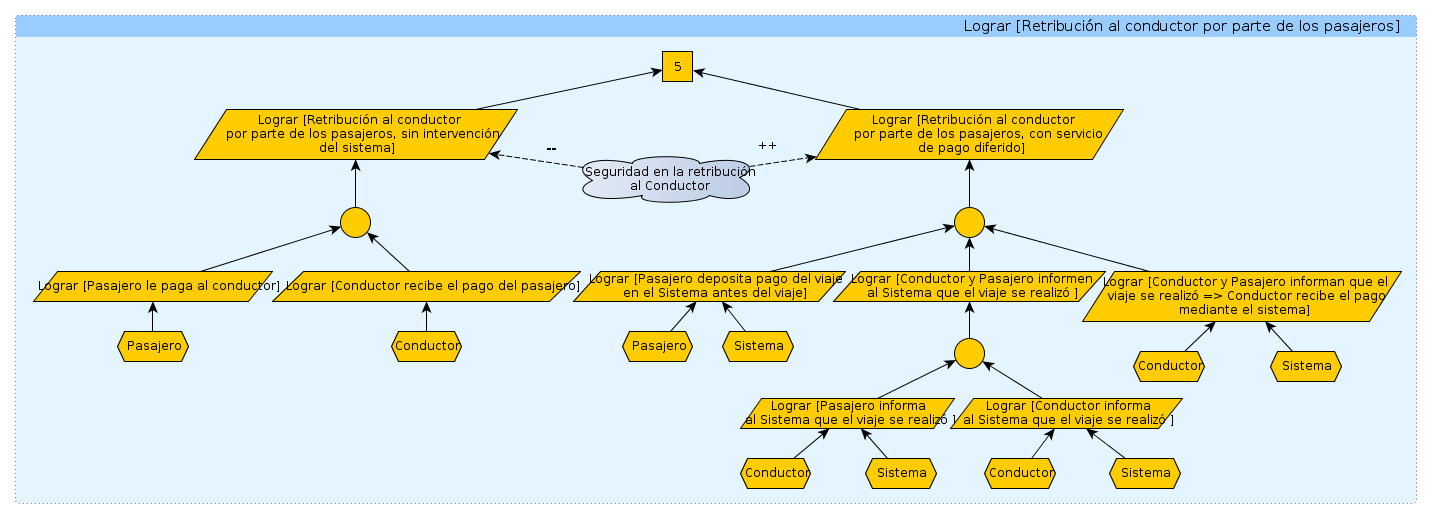
\includegraphics[height=7cm,width=19.5cm]{imagenes/Retribucion.png}

\subsection{Informaci�n}
a\\
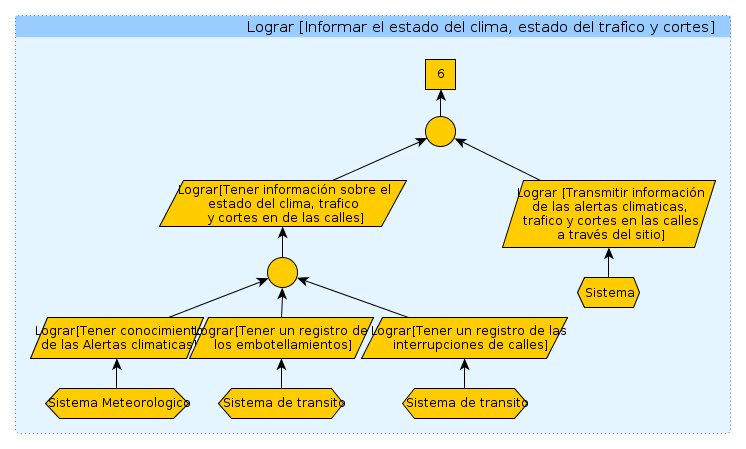
\includegraphics[height=7cm,width=19.5cm]{imagenes/InformacionDelClimayViajes.png}



\newpage

\section{Escenarios} %Escribir los escenarios
Aqu� detallaremos algunos de los posibles escenarios del sistema de Carpooling

\subsection{Escenario 1}
Javier Baez, es un trabajador de una empresa que queda en el centro de cambodia, todos los dias se levanta muy temprano para ir a trabajar
porque lamentablemente la cantidad de autos que van hacia el mismo lugar es muy alta, utiliza el mismo recorrido todos los dias truene o salga el sol.
Es en uno de sus viajes al trabajo observa que el conductor del auto de su costado es un compa�ero de trabajo, Alberto, y que estan junto a el otras 3 personas que nunca habia visto.
Cuando llega al trabajo, lo ve sin ninguna compa�ia y por curiosidad le pregunta quienes eran sus acompa�antes, este responde que los conoci� a travez del programa de carpooling promocionado por el gobierno, sin entender de que se trata, Javier le pregunta la razon por la que utiliza el programa de carpooling y si no le asustaba que se suban extra�os en su auto, este responde que de esa manera disminuyen la cantidad de automoviles en la calle lo que afecta directamente al trafico que hay en su recorrido al trabajo y que el sistema le permite aceptar o no al solicitante que va a subirse a su automovil. Sorprendido por la respuesta, Javier se da cuenta de que existe una solucion a los problemas de trafico que tiene que lidiar todos los dias y decide entrar al sitio del gobierno para conocer mejor el funcionamiento del carpool, es asi como cuando llega a su oficina descubre que el sistema planteado le permite seleccionar quienes viajarian con el, de manera que el se sienta seguro, y que muchas otras personas conocidas ya participan del programa, ademas, advierte algo que su compa�ero no le habia informado, no solamente el sistema le permitiria reducir el tiempo en realizar su recorrido sino que tambi�n los usuarios le pagarian a el por transportarlos lo que reduciria una parte de sus gastos diarios. Entusiasmado, rapidamente se registra en el programa como conductor, ingresa su recorrido y costo y vuelve a trabajar. Al finalizar su horario de trabajo, ingresa al sitio para verificar si alg�n pasajero desea volver con el y para su sorpresa son 5 los solicitantes, de ah� Javier elige a 3, se comunica con ellos a travez del sistema, se aceptan mutuamente y establecen la forma de pago. Todo funciona a la perfecci�n y Javier vuelve muy contento a su casa.

Al llegar a su casa, Javier le comenta a su mujer, Marina, de su descubrimiento, ella, como usuario del transporte publico se ve muy interesada en algo que le permita evitar las largas horas de viaje parada lo que le resulta muy incomodo y molesto para ir a trabajar, es asi que decide investigar un poco de que se trata el sistema.
Luego de registrarse descubre en el que existen muchos Conductores que realizan viajes parecidos al de ella y con un costo que ella considera correcto, entonces decide enviar la solicitud a un conductor, est� se pone en contacto con ella y se ponen de acuerdo para ir juntos al dia siguiente.
Al dia siguiente, el dia del viaje, Marina decide entrar al sistema para abonar el viaje y advierte que la ruta acordada estaba intervenida por unos empleados en huelga, es asi que se pone en contacto con el Conductor y deciden modificar el recorrido, en ese mismo momento el conductor advierte al resto de los pasajeros del cambio de recorrido y el viaje se realiza de forma correcta y sin inconvenientes de trafico.
Luego de este viaje, Marina se siente muy satisfecha con el sistema y se lo comenta a todos sus compa�eros de trabajo.

\end{document} %Termin�!

